\section[Intruduction]{Introduction au domaine}


\subsection[E-Ink]{Technologie E-Ink}
\begin{frame}{Technologie E-Ink}
	%% A compléter par Arthur
\end{frame}


\subsection[Sony PRS-T1]{Liseuse Sony PRS-T1}
\begin{frame}{Caractéristiques principales} %% Liseuse en générale
		\begin{itemize}
			\item Processeur iMX508
			\item Écran E-Ink 6 pouces
			\item Résolution jusqu'à 16 niveaux de gris
			\item Interfaces USB
			\item WiFi
			\item Mémoire : 2Go (extensible par microSD)
		\end{itemize}
\end{frame}

\begin{frame}{Processeur iMX508} %% partie iMX508
	\begin{itemize}
		\item{Développé par Freescale}
		\item{Architecture ARM Cortex A8}
		\item{Faible consommation d'énergie}
		\item{Bonnes performances}
		\item{Contrôleur d'écran intégré}
		
	\end{itemize}
\end{frame}

\begin{frame}{Modules}
	\begin{itemize}
		\item{EPDC}
		\begin{itemize}
			\item{Dirige les signaux (waveform)}
			\item{Mise à jour partielle ou totale}
		\end{itemize}
		\item{ePXP}
		\begin{itemize}
			\item Transparence
			\item Rotation d'image
			\item Agrandissement / Réduction d'image
		\end{itemize}
	\end{itemize}
\end{frame}

\begin{frame}{Architecture du processeur iMX508} %% Schéma
	\begin{figure}
		\begin{center}
			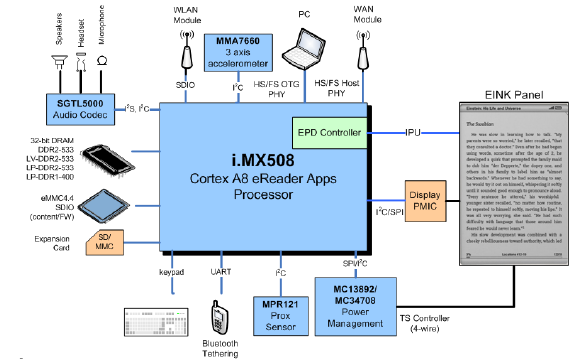
\includegraphics[scale=0.65]{iMX508.png}
		\end{center}
	\end{figure}
\end{frame}

\begin{frame}{Hack de la liseuse}
		\begin{itemize}
			\item{Débloquer la liseuse}
			\item{Plusieurs méthodes :}
			\begin{itemize}
				\item{Mise à jour du firmware}
				\item{Mode Recovery}
			\end{itemize}
		\end{itemize}
\end{frame}
